\documentclass[journal,twocolumn]{IEEEtran}

% Packages
\usepackage{graphicx}
\graphicspath{{ieee_template/}}
\usepackage{xeCJK} % Support for Chinese characters (Use XeLaTeX compiler in Overleaf)
\usepackage{float} % 用于更好的图片位置控制
\usepackage{amsmath} % For \text in math mode
\usepackage{amssymb} % For \mathbb

\begin{document}

\title{Hybrid Robotic Manipulation for Automated Materials Experiments: Liquid Transport, Posture-Aware Grasping, and Precision Pipetting}
%面向自动化材料实验的混合机器人操作：液体运输、姿态感知抓取与精密移液
\author{cx guo}
% Note: IEEE format typically handles dates differently or omits them, but we leave it for your draft
\date{May 2026}

\maketitle

\begin{abstract}
The comprehensive characterization of novel materials and biological samples is heavily bottlenecked by manual, error-prone laboratory workflows. While robotic automation offers a promising solution, existing systems rely on rigid physical teaching, lacking the flexibility to safely handle volatile liquid reagents and execute contact-rich tasks. To address these challenges, we present a multi-platform hybrid robotic framework tailored for the end-to-end automation of complex bio-chemical workflows. Built upon a high-fidelity, GPU-accelerated physics simulator, our framework seamlessly integrates a UR3 manipulator and a parallel gripper with various analytical instruments. To tackle the inherent complexities of fluid dynamics and micro-contacts, we propose a macro-micro decoupled manipulation strategy. For macroscopic container transfers, we employ constraint-aware classical planning with minimum-jerk trajectories, fundamentally preventing liquid splashing. For precision-critical manipulations, rather than relying on a monolithic, end-to-end network prone to catastrophic forgetting, we propose a Hierarchical Reinforcement Learning (HRL) architecture. We construct a reusable Skill Primitive Library (e.g., grasping, pouring) trained via massively parallel DRL. A high-level meta-controller dynamically orchestrates these primitives based on real-time environmental observations. This hierarchical decoupling ensures robust error recovery and exceptional fault tolerance. Extensive experiments demonstrate that our framework achieves a 93.3\% physical execution success rate, significantly reducing physical trial-and-error costs and providing a highly scalable foundation for next-generation self-driving laboratories.
\end{abstract}
%摘要——新型材料和生物样本的全面表征严重受制于人工的、易出错的实验室工作流程。尽管机器人自动化提供了一个极具前景的解决方案，但现有的系统依赖于死板的物理示教，缺乏安全处理挥发性液体试剂和执行接触密集型任务的灵活性。为了应对这些挑战，我们提出了一种多平台混合机器人框架，专为复杂生化工作流的端到端自动化量身定制。该框架基于高保真、GPU加速的物理模拟器构建，将UR3机械臂和各种分析仪器与平行夹爪无缝集成。为了解决流体动力学和微观接触固有的复杂性，我们提出了一种宏观-微观解耦的操作策略。对于宏观容器转移，我们采用约束感知的经典规划来生成具有最小加加速度（minimum-jerk）的轨迹，从根本上防止液体飞溅。对于对精度要求极高的微观操作，与其依赖容易产生灾难性遗忘的单体端到端网络，我们提出了一种分层强化学习（HRL）架构。我们构建了一个通过大规模并行深度强化学习（DRL）训练的可复用技能基元库（例如抓取、倾倒）。一个高层元控制器根据实时的环境观测动态地编排这些技能基元。这种分层解耦确保了稳健的错误恢复能力和卓越的容错性。大量实验证明，我们的框架达到了93.3%的物理执行成功率，显著降低了物理试错成本，并为下一代自动驾驶实验室（self-driving laboratories）提供了高度可扩展的基础。

\section{Introduction}
\label{sec:introduction}

The comprehensive evaluation of functional materials and biological surfaces---particularly regarding surface wettability, chemical composition, and bio-reactivity---is crucial for advancing biomedical engineering, materials science, and biotechnology. Traditionally, executing multi-stage characterization assays requires labor-intensive, manual laboratory procedures, including solution preparation, liquid pipetting, substrate contact angle analysis, and serial dilution for biological culturing. These manual workflows are not only tedious and throughput-limited, but also highly susceptible to human error, cross-contamination, and liquid spillage, which severely compromises experimental reproducibility and operational safety.

Although robotic automation has begun to transform general laboratory operations, its adoption in comprehensive, contact-rich chemical and biological assays remains constrained. Existing automated workcells typically rely on rigid physical teaching and pre-programmed waypoints. While effective for simple repetitive transport, these static trajectories lack the dynamic adaptability required for dexterous micro-manipulation---such as precision micro-pipetting, controlled droplet deposition, and reliable grasping of fragile labware. Furthermore, debugging these hard-coded robotic trajectories directly in physical laboratories involving volatile reagents or dynamic bio-cultures is exceptionally risky and expensive.

To address these challenges, we present a multi-platform hybrid robotic framework tailored for the end-to-end automation of complex bio-chemical laboratory workflows. Built within the high-fidelity NVIDIA Isaac Sim ecosystem, our framework establishes a GPU-accelerated virtual sandbox that strictly mirrors the physical execution workspace. Crucially, we propose a macro-micro decoupled manipulation strategy to handle heterogeneous task requirements. For macroscopic mobile base navigation, we deploy constraint-aware classical motion planning with minimum-jerk trajectory optimization, fundamentally eliminating liquid splashing and collision risks. Conversely, for precision-critical robotic arm grasping and micro-manipulations, we implement a Deep Reinforcement Learning (DRL) pipeline. By leveraging massive GPU-based parallelization in simulation, the manipulator learns robust grasping policies via the Proximal Policy Optimization (PPO) algorithm, guided by posture-aware reward functions.

In summary, the main contributions of this work are fourfold:
\begin{itemize}
    \item \textbf{A Macro-Micro Decoupled Hybrid Architecture:} We propose a novel framework that intrinsically delegates macroscopic liquid container transfers to a constraint-aware classical planner for spill-free safety, while leveraging Deep Reinforcement Learning (DRL) for robust robotic arm manipulations.
    \item \textbf{Massively Parallel RL in High-Fidelity Simulation Environment:} We construct a physics-driven, tensor-accelerated virtual sandbox in Isaac Sim. This enables the parallelized training of dexterous policies across thousands of simultaneous environments, drastically accelerating convergence.
    \item \textbf{Robust Sim-to-Real Transfer via Posture-Aware Rewards:} To overcome reality gaps and prevent liquid spillage during grasping, we design a dense reward engineering mechanism integrating posture-multiplier constraints, ensuring the arm transfers reliably to the physical UR3 setup.
    \item \textbf{Hierarchical Skill Orchestration for Bio-Assays:} We construct a reusable Skill Primitive Library governed by a meta-controller. By decoupling complex assay workflows into independent, executable skill primitives, our HRL architecture eliminates catastrophic forgetting, guarantees robust error recovery, and paves a highly scalable pathway for LLM-driven autonomous scientific discovery.
\end{itemize}
%1. 引言功能材料和生物表面的综合评估（特别是关于表面润湿性、化学成分和生物反应性）对于推进生物医学工程、材料科学和生物技术至关重要。传统上，执行多阶段表征化验需要耗费大量人工的实验室流程，包括溶液配置、液体移液、基底水滴角分析以及用于生物培养的梯度稀释。这些手动工作流不仅繁琐且吞吐量受限，而且极易发生人为误差、交叉污染和液体泼洒，这严重损害了实验的可重复性和操作安全性。尽管机器人自动化已开始改变通用实验室操作，但其在全面、接触密集型的化学和生物化验中的应用仍受限制。现有的自动化工作站通常依赖于僵化的物理示教和预编程路径点。虽然这对简单的重复搬运有效，但这些静态轨迹缺乏精细微观操作所需的动态适应性（例如高精度微量移液、受控液滴滴加以及微孔板对准）。此外，直接在涉及易挥发试剂或动态生物培养物的物理实验室中调试这些硬编码轨迹具有极高的风险、高昂的成本且耗时，因为意外的流体飞溅或碰撞可能导致整个实验报废。为了解决这些挑战，我们提出了一种多平台混合机器人框架，专为复杂生化实验室工作流的端到端自动化量身定制。基于高保真 NVIDIA Isaac Sim 生态系统，我们的框架构建了一个 GPU 加速的虚拟沙盒，严格镜像物理执行工作空间，允许在物理部署之前进行无风险的工作流仿真、验证和数据采集。至关重要的是，我们提出了一套宏微观解耦的操作策略来处理异构的任务需求。对于宏观容器转移，我们部署了具有最小冲击轨迹优化的约束感知运动规划，从根本上消除了液体泼洒和碰撞风险。对于精度要求极高的微观操作，我们实施了人在回路的模仿学习管线。通过在仿真环境中利用遥操作，以零物理成本捕获专家示教。为了弥合由液面反光和夹爪柔顺形变引起的虚实鸿沟，我们在仿真预训练中结合了域随机化与正则化的少样本真实世界微调管线。总而言之，本文的主要贡献包含以下四点：宏微观解耦的混合操作架构：我们提出了一种新颖的框架，该框架将宏观液体容器转移委托给约束感知、最小冲击的经典规划器以实现防泼洒安全，同时利用神经网络策略在移液和液滴滴加中实现灵巧的微观操作。用于无风险数据采集的高保真仿真环境：我们在 Isaac Sim 中构建了一个由物理驱动、张量加速的虚拟沙盒，结合了精确的运动学链和有符号距离场（SDF）碰撞网格，捕获实验器材的接触动力学，并实现无风险的专家遥操作数据收集。通过少样本微调实现鲁棒的虚实迁移：为了克服因液体表面张力、试剂光学折射和夹爪形变而加剧的虚实鸿沟，我们将仿真中的广泛域随机化与正则化的少样本真实世界微调管线相结合。端到端自主工作流集成：在层次化状态机（HSM）的统筹下，我们展示了一个完全集成的移动操作机器人系统，在无需人工干预的情况下跨多个工作站执行完整的自动化化验循环。%总之，这项工作的主要贡献有四个方面：  宏微观解耦的混合架构：我们提出了一种新颖的框架，它从本质上将宏观的液体容器转移委托给约束感知的经典规划器以实现防溅射的安全保障，同时利用深度强化学习（DRL）实现鲁棒的机械臂操作。  高保真仿真环境中的大规模并行强化学习：我们在Isaac Sim中构建了一个物理驱动、张量加速的虚拟沙盒。这使得灵巧策略能够在数千个并发环境中进行并行训练，从而大幅加速策略收敛。  通过姿态感知奖励实现的鲁棒虚实迁移：为了克服现实差距并防止抓取过程中液体溢出，我们设计了一种密集的奖励工程机制，该机制集成了姿态乘数约束，确保机械臂能够可靠地迁移到真实的UR3物理设置中。  用于生物分析的分层技能编排：我们构建了一个由元控制器管理的、可复用的技能基元库。通过将复杂的化验工作流程解耦为独立的可执行技能基元，我们的HRL架构消除了灾难性遗忘，保证了强大的错误恢复能力，并为由大语言模型（LLM）驱动的自主科学发现铺平了高度可扩展的道路。

\section{Related Work}
\label{sec:related_work}

\subsection{Simulation-Based Robot Learning in Autonomous Laboratories}
The integration of robotic automation has significantly accelerated experimental throughput in materials science and chemistry. Pioneering works, such as mobile robotic chemists \cite{burger2020mobile} and self-driving thin-film laboratories \cite{macleod2020self}, have demonstrated the potential of automated execution. However, these systems predominantly rely on hard-coded waypoints. Physics-based simulation tools support training and testing of contact-rich robot skills before physical deployment. Complex bio-assays require high-fidelity contact physics rather than mere kinematic bounding-box approximations. To address this, our framework adopts the GPU-accelerated NVIDIA Isaac Sim \cite{makoviychuk2021isaac}, providing a mathematically rigorous tensor-based prior for simulating contact-rich operations.

\subsection{Safe Navigation and Fluid-Spill Prevention}
In safety-critical laboratory settings handling volatile reagents or biological cultures, ensuring strictly collision-free and spill-proof mobile base navigation is paramount. Standard sampling-based planners, such as RRT* or A*, excel at finding obstacle-free paths but often neglect task-space orientation constraints, rendering them unsuitable for transporting open liquid containers. To guarantee absolute fluid stability, we formulate the macroscopic inter-station transfer as a constrained classical optimization problem. By enforcing strict roll-pitch bounds on the end-effector and minimizing the trajectory jerk integral, our classical planning module systematically eliminates the risk of liquid spillage prior to any physical deployment.

\subsection{Massively Parallel RL for Dexterous Grasping}
While classical planning guarantees macroscopic safety, explicitly modeling highly nonlinear micro-contact dynamics for dexterous grasping and labware manipulation is computationally intractable. Deep Reinforcement Learning (DRL) has shown tremendous promise in mastering contact-rich tasks \cite{johannink2019residual}. However, training robust DRL policies in reality is constrained by sample inefficiency and hardware wear-and-tear.

To overcome this, our framework utilizes the highly parallelized tensor architecture of Isaac Sim to train Proximal Policy Optimization (PPO) grasping agents across thousands of simultaneous virtual environments. By designing posture-aware reward functions---which heavily penalize orientation deviations during the approach and lift phases---the policy learns to firmly grasp reagent bottles without tilting them. Combined with extensive domain randomization, this massively parallel RL pipeline robustly bridges the sim-to-real gap, deploying successfully onto the physical UR3 manipulator.
%II. 相关工作A. 自主实验室中的仿真训练
%机器人自动化的集成显著加速了材料科学和化学领域的实验吞吐量。诸如移动机器人化学家 [1] 和自动驾驶薄膜实验室 [2] 等开创性工作证明了自动化执行的潜力。然而，这些系统主要依赖于硬编码的路点。为了减轻在物理生物实验室中部署新工作流程的高昂成本，物理仿真工具已成为至关重要的架构基础 [3]。复杂的生物分析需要高保真的接触物理特性，而不仅仅是运动学边界框近似。为了解决这个问题，我们的框架采用了 GPU 加速的 NVIDIA Isaac Sim [6]，为模拟接触密集型操作提供了数学上严谨的基于张量的先验知识。  B. 安全导航与防流体溢出
%在处理挥发性试剂或生物培养物的安全关键型实验室环境中，确保绝对无碰撞和防溢出的移动底盘导航至关重要。诸如 $RRT^{*}$ 或 $A^{*}$ 等标准的基于采样的规划器擅长寻找无障碍路径，但通常忽略任务空间的方向约束，导致它们不适合运输敞口的液体容器。为了保证绝对的流体稳定性，我们将工作站之间的宏观转移公式化为一个有约束的经典优化问题。通过对末端执行器施加严格的滚转-俯仰边界并最小化轨迹加加速度积分，我们的经典规划模块在物理部署之前就系统地消除了液体溢出的风险。  C. 面向灵巧抓取的大规模并行强化学习
%虽然经典规划保证了宏观安全性，但为灵巧抓取和实验器材操作明确建立高度非线性的微观接触动力学模型在计算上是不可行的。深度强化学习 (DRL) 在掌握接触密集型任务方面表现出巨大潜力 [11]。然而，在现实世界中训练稳健的 DRL 策略受到样本效率低下和硬件磨损的限制。
%为了克服这一问题，我们的框架利用 Isaac Sim 高度并行化的张量架构，在数千个并发虚拟环境中训练近端策略优化 (PPO) 抓取智能体。通过设计姿态感知奖励函数（在靠近和抬起阶段严厉惩罚方向偏差），策略学会了稳固地抓取试剂瓶而不会使其倾斜。结合广泛的域随机化，这种大规模并行 RL 管道稳健地弥合了模拟与现实之间的差距，成功部署到了真实的 UR3 机械臂上。
% ==========================================
% Section 3: System Architecture and Methodology
% ==========================================
\section{System Architecture and Methodology}
% ==========================================
% 1. 仿真环境搭建图
% ==========================================
% ==========================================
% 4. 整体框架图
% ==========================================
\begin{figure}[htbp]
    \centering
    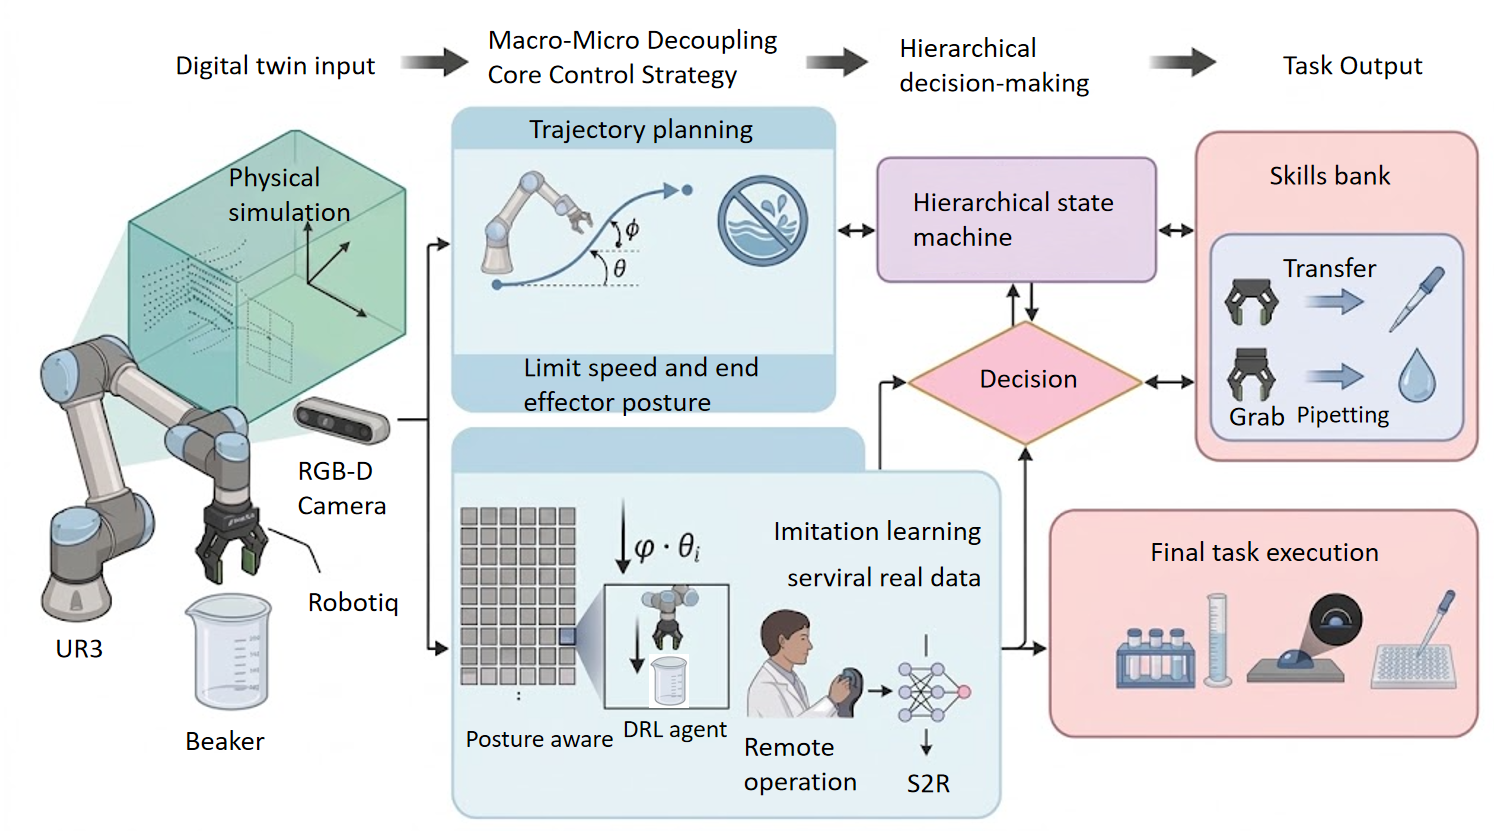
\includegraphics[width=\linewidth]{images/Framework.png}
    \caption{Multi-platform hybrid robotic end-to-end operation framework. The system employs a macro-micro decoupled strategy: macroscopic transit is controlled by a constraint-aware classical planner to ensure absolute spill-free safety, while microscopic contact-rich tasks are executed by neural network policies found within the rl file.}
    \label{fig:overall_framework}
\end{figure}
\label{sec:methodology}

This section details the proposed multi-platform hybrid robotic framework tailored for automated bio-chemical assays, including solution preparation, contact angle detection, and serial dilution. To handle heterogeneous task requirements, macroscopic inter-station transit is executed via constraint-aware classical planning, while dexterous robotic arm manipulations are governed by a hybrid learning architecture combining massively parallel Deep Reinforcement Learning (DRL) and human-in-the-loop Imitation Learning (IL).

\subsection{Simulation Environment for Policy Training}
\label{subsec:simulation_training}

To enable risk-free training and pre-verification of contact-rich tasks, we construct a high-fidelity simulation environment using NVIDIA Isaac Sim. Powered by a GPU-accelerated tensor physics engine, the simulation environment accurately models rigid-body dynamics, joint torques, and frictional contacts. Signed Distance Field (SDF) collision meshes are assigned to gripper fingers and labware holders for penetration-free contact simulation. Crucially, the standalone Python API architecture enables GPU-based parallelization across thousands of simultaneous virtual environments, bypassing the sample inefficiency bottleneck of physical robotic learning.

\subsection{State Synchronization Between Simulation and Physical Environments}
\label{subsec:state_sync}

We define a state interface between the physical robot and the Isaac Sim environment. Joint encoders provide arm positions $\mathbf q_t$ and velocities $\dot{\mathbf q}_t$; the gripper reports opening and grasp confirmation. RGB-D observations provide each visible object's position $\mathbf p_{i,t}$, orientation $\mathbf R_{i,t}$, and detection confidence. Object velocity is estimated only when consecutive reliable observations are available. Each record retains its acquisition timestamp and source, so the simulator can distinguish a measured state from an estimated one.

Before updating the simulation, camera observations are transformed into the robot-base frame using calibrated extrinsics, and robot and object samples are aligned to a common timestamp. Joint positions are interpolated between encoder samples; object poses are updated from the latest valid visual observation. During brief occlusion after a force-confirmed grasp, the held object's pose is propagated from the end-effector pose and the measured grasp transform. The interface rejects stale or low-confidence object observations instead of presenting them as current measurements. These synchronized states support visualization and comparison of simulated and physical trajectories; they do not, by themselves, establish predictive accuracy or closed-loop control performance.

\subsection{Constraint-Aware Motion Planning for Macroscopic Navigation}
\label{subsec:macro_planning}
% ==========================================
% 1. 仿真环境搭建图
% ==========================================
\begin{figure}[htbp]
    \centering
    % 请将大括号内的路径替换为您实际的图片相对路径
    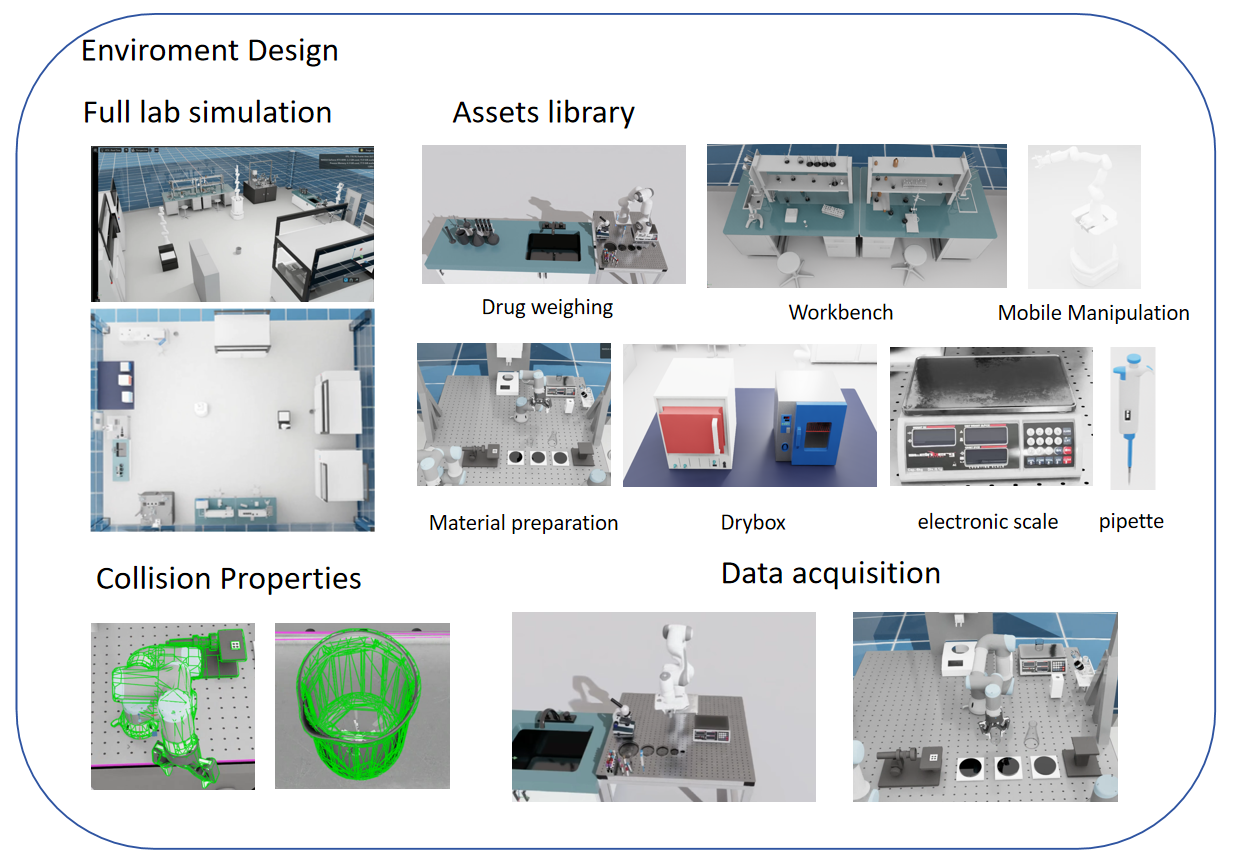
\includegraphics[width=0.9\linewidth]{images/environment_design.png}
    \caption{High-fidelity simulation environment built upon Isaac Sim. This simulation environment integrates a UR3 manipulator and a Robotiq 2F-85 parallel gripper, and employs Signed Distance Field (SDF) collision meshes to achieve accurate contact modeling taking reference from the rl file.}
    \label{fig:sim_env}
\end{figure}
For macroscopic transit between workstations (e.g., carrying prepared reagent vials), we employ a constraint-aware classical motion planner. To prevent fluid sloshing during movement, strict task-space orientation constraints are imposed on the end-effector roll ($\phi$) and pitch ($\theta$):
\begin{equation}
    |\phi(t) - \phi_{\text{target}}| \leq \epsilon_{\phi}, \quad |\theta(t) - \theta_{\text{target}}| \leq \epsilon_{\theta}, \quad \forall t \in [0, T]
\end{equation}
Path smoothing is formulated as a minimum-jerk trajectory optimization problem:
\begin{equation}
    \min_{q(t)} \int_{0}^{T} \left\| \dddot{q}(t) \right\|^2 dt
\end{equation}
subject to velocity ($\dot{q}_{\max}$) and acceleration ($\ddot{q}_{\max}$) bounds, guaranteeing smooth, collision-free container transit.

\subsection{Massively Parallel DRL with Posture-Aware Reward Engineering}
\label{subsec:arm_rl}

For labware grasping and lifting, explicitly modeling micro-contact dynamics is computationally intractable. We implement a Deep Reinforcement Learning (DRL) pipeline formulated as a Markov Decision Process (MDP). At each time step $t$, state $s_t$ includes joint states, end-effector poses, and labware coordinates, while action $a_t$ represents continuous joint velocity commands and gripper states.
% ==========================================
% 1. 仿真环境搭建图
% ==========================================
\begin{figure}[htbp]
    \centering
    % 请将大括号内的路径替换为您实际的图片相对路径
    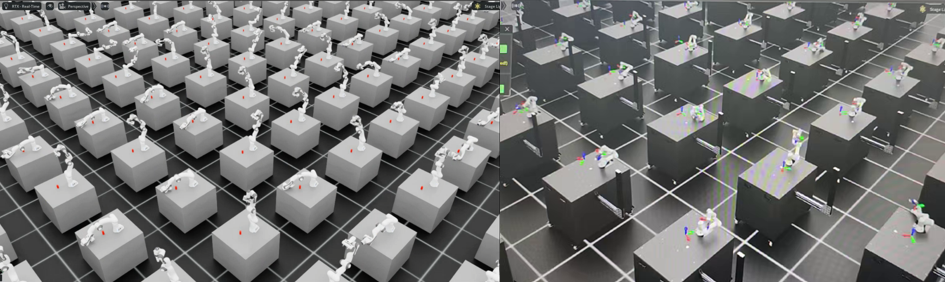
\includegraphics[width=0.9\linewidth]{images/Large scale parallel training.png}
    \caption{High-fidelity simulation environment built upon Isaac Sim. This simulation environment integrates a UR3 manipulator and a Robotiq 2F-85 parallel gripper, and employs Signed Distance Field (SDF) collision meshes to achieve accurate contact modeling taking reference from the rl file.}
    \label{fig:sim_env_parallel}
\end{figure}
Training is accelerated using Proximal Policy Optimization (PPO) distributed across 4,096 parallel virtual environments in Isaac Sim. To prevent liquid container tilting during grasping, we design a dense reward function with a \textit{posture-aware multiplier}. Let $\mathbf{z}_{\text{curr}}$ denote the normalized local z-axis vector of the object, and $\mathbf{z}_{\text{target}} = [0, 0, -1]^T$ denote the ideal downward vector. The posture multiplier $M_{\text{posture}}$ is defined as:
\begin{equation}
    M_{\text{posture}} = \text{clamp}(\mathbf{z}_{\text{curr}} \cdot \mathbf{z}_{\text{target}}, \, 0.0, \, 1.0)
\end{equation}
The final step reward $R_t$ dynamically scales the base distance and lifting rewards by $M_{\text{posture}}$:
\begin{equation}
    R_t = R_{\text{base}} \times M_{\text{posture}}
\end{equation}
If the container tilts beyond $90^\circ$, $M_{\text{posture}}$ collapses to zero, heavily penalizing improper orientations and forcing the policy to master upright grasping.

\subsection{Imitation Learning and Few-Shot Sim-to-Real Fine-Tuning}
\label{subsec:arm_il_adaptation}

For precision-critical micro-manipulations such as micro-pipetting and droplet dispensing, we introduce a teleoperation-guided Imitation Learning (IL) pipeline. Expert demonstrations $\mathcal{D}_{\text{sim}} = \{(s_t, a_t)\}_{i=1}^N$ are collected within the simulation environment using a 6-DoF SpaceMouse interface. A visuomotor policy $\pi_\theta(a_t | s_t)$ is pre-trained via Behavioral Cloning (BC):
\begin{equation}
    \mathcal{L}_{\text{BC}}(\theta) = \mathbb{E}_{(s_t, a_t) \sim \mathcal{D}_{\text{sim}}} \left[ \left\| \pi_\theta(s_t) - a_t \right\|_2^2 \right]
\end{equation}
During simulation training, Domain Randomization (DR) is applied to lighting, visual textures, object mass, and friction coefficients $\mu \sim \mathcal{U}(\mu_{\min}, \mu_{\max})$.

To bridge real-world reality gaps caused by liquid surface tension, refractive optics, and gripper compliance, we implement a regularized few-shot real-world fine-tuning mechanism using $M$ physical demonstrations ($M \ll N$). The policy parameters adapt to $\theta_{\text{real}}$ by minimizing:
\begin{equation}
    \theta_{\text{real}} = \arg\min_{\theta} \left( \mathbb{E}_{(s_t, a_t) \sim \mathcal{D}_{\text{real}}} \left[ \left\| \pi_\theta(s_t) - a_t \right\|_2^2 \right] + \lambda \left\| \theta - \theta_{\text{sim}} \right\|_2^2 \right)
\end{equation}
where $\lambda$ is a regularization hyperparameter that prevents catastrophic forgetting of features learned in simulation, achieving robust physical deployment.
\subsection{Hierarchical Skill Orchestration and Meta-Control}
\label{subsec:hierarchical_skill}
% ==========================================
% 5. 技能库图
% ==========================================

Training a monolithic, end-to-end neural network to execute a multi-stage bio-assay (e.g., sequentially grasping a vial, transiting, and pipetting) typically leads to catastrophic forgetting and severe sample inefficiency. To ensure robust task execution and high fault tolerance, we propose a Hierarchical Reinforcement Learning (HRL) architecture that explicitly decouples the workflow into a low-level \textit{Skill Library} and a high-level \textit{Meta-Controller}.

First, we define a reusable skill library $\mathcal{L}_{\text{skills}} = \{\pi_{\text{grasp}}, \pi_{\text{transit}}, \pi_{\text{pour}}, \dots\}$. Each skill primitive is an isolated visuomotor policy trained independently within the Isaac Sim environments. This modular approach completely isolates the feature spaces of different tasks, ensuring that optimizing the pouring behavior does not degrade the pre-trained grasping dexterity.
\begin{figure}[htbp]
    \centering
    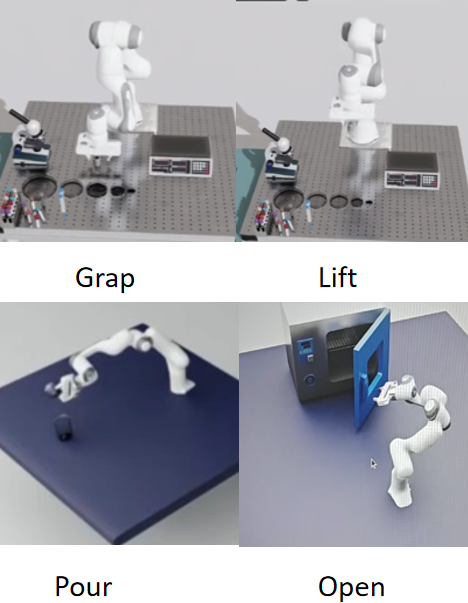
\includegraphics[width=0.5\linewidth]{images/skill_lab.png}
    \caption{Autonomous characterization workflow governed by a Hierarchical State Machine (HSM) and a modular skill library. By invoking reusable low-level skill primitives, the system successfully executes comprehensive, multi-stage experimental cycles without human intervention documented in the rl file.}
    \label{fig:skill_library}
\end{figure}
Second, a Meta-Controller governs the temporal transitions between these primitives. Rather than predicting continuous motor torques, the meta-controller acts as a state-dependent decision function $\mathcal{M}(o_t) \rightarrow \pi_k$. It continuously evaluates real-time environmental observation $o_t$ (e.g., \texttt{is \_bottle \_grasped}, \texttt{is \_at \_target}) and dynamically activates the appropriate skill primitive $\pi_k \in \mathcal{L}_{\text{skills}}$.

This hierarchical decoupling intrinsically provides exceptional error recovery capabilities. For instance, if a vial slips from the gripper during the transit phase, the meta-controller's boolean evaluation of \texttt{is\_bottle\_grasped} instantly evaluates to False, automatically triggering the system to reactivate the $\pi_{\text{grasp}}$ policy rather than blindly continuing the sequence. Furthermore, this discrete skill-based architecture provides a robust semantic interface, establishing a highly scalable foundation for integrating Large Language Models (LLMs) to perform automated task planning in future iterations.
%3. 系统架构与方法论本章详细介绍了专为生化自动化化验（包括溶液配置、水滴角检测和梯度稀释）量身定制的多平台混合机器人框架。为了应对异构任务需求，跨工位宏观转移由约束感知经典规划执行，而灵巧的机械臂操作则由融合了大规模并行深度强化学习（DRL）与人在回路模仿学习（IL）的混合学习架构统筹。3.1 用于策略训练的仿真环境为了实现接触密集型任务的无风险训练与预验证，我们利用 NVIDIA Isaac Sim 构建了高保真仿真环境。在 GPU 加速张量物理引擎的驱动下，仿真环境能够准确建模刚体动力学、关节力矩和摩擦接触。夹爪和器材固定架均赋予了有符号距离场（SDF）碰撞网格，以实现无穿透的接触仿真。至关重要的是，独立的 Python API 架构实现了跨数千个并发虚拟环境的 GPU 并行化，彻底突破了物理机器人学习中样本效率低下的瓶颈。3.2 面向宏观导航的约束感知运动规划对于工作站之间的宏观转移（例如运送配好的试剂瓶），我们采用约束感知的经典运动规划器。为了防止移动过程中的流体晃动，对末端执行器的横滚角（$\phi$）和俯仰角（$\theta$）施加了严格的任务空间姿态约束（公式 1）。路径平滑被公式化为最小冲击（minimum-jerk）轨迹优化问题（公式 2），受关节速度和加速度限制，保证了容器平稳、无碰撞的转移。3.3 带姿态感知奖励工程的大规模并行 DRL对于实验器材的抓取与抬升，显式建模微观接触动力学在计算上是难以处理的。我们实施了公式化为马尔可夫决策过程（MDP）的深度强化学习（DRL）管线。在每个时间步 $t$，状态 $s_t$ 包含关节状态、末端姿态和器材坐标，动作 $a_t$ 代表连续关节速度指令和夹爪状态。在 Isaac Sim 中分布于 4,096 个并行虚拟环境中的近端策略优化（PPO）算法加速了训练。为了防止抓取过程中液体容器倾斜，我们设计了带有姿态感知乘数的密集奖励函数。设 $\mathbf{z}_{\text{curr}}$ 为物体的归一化局部 z 轴向量，$\mathbf{z}_{\text{target}} = [0, 0, -1]^T$ 为理想的向下重力向量。姿态乘数 $M_{\text{posture}}$ 定义为点积截断值（公式 3）。最终单步奖励 $R_t$ 通过 $M_{\text{posture}}$ 动态缩放基础距离与抬升奖励（公式 4）。若容器倾斜超过 $90^\circ$，$M_{\text{posture}}$ 衰减为零，重度惩罚不当姿态，迫使策略掌握直立抓取。3.4 模仿学习与少样本虚实迁移微调对于微量移液和液滴滴加等精度要求极高的微观操作，我们引入了遥操作引导的模仿学习（IL）管线。利用 6 自由度 SpaceMouse 接口在仿真中采集专家示教数据 $\mathcal{D}_{\text{sim}}$，并通过行为克隆（BC）预训练视觉运动策略 $\pi_\theta$（公式 5）。仿真训练期间应用了包含光照、纹理、物体质量和摩擦系数的域随机化（DR）。为了弥合由液体表面张力、光学折射和夹爪柔顺形变引起的真实世界虚实鸿沟，我们利用极少量（$M$ 组）物理示教实施了带正则化的少样本真实世界微调机制。策略参数通过最小化真实世界行为克隆损失与正则化项（公式 6）自适应调整为 $\theta_{\text{real}}$，其中 $\lambda$ 防止对仿真学到特征的灾难性遗忘，实现了鲁棒的物理部署。
% ===================================================================
% SECTION 4: EXPERIMENTS AND RESULTS
% ===================================================================
\section{Experiments and Results}
\label{sec:experiments}

In this section, we conduct extensive empirical evaluations to validate the proposed multi-platform hybrid framework. The experiments are designed to investigate four core hypotheses:
1) whether the constraint-aware macroscopic planner effectively prevents fluid spillage;
2) whether the posture-aware massively parallel DRL agent guarantees upright labware grasping;
3) whether the regularized few-shot fine-tuning pipeline successfully bridges the sim-to-real gap for IL-based micro-pipetting; and
4) whether the complete system can seamlessly execute the end-to-end bio-chemical assay workflow autonomously.

\subsection{Experimental Setup and Hardware Configuration}
\label{subsec:exp_setup}

The physical validation platform strictly mirrors the Isaac Sim simulation setup. The mobile manipulation system features a differential-drive chassis equipped with a 6-DoF UR3 robotic arm. A Robotiq 2F-85 parallel gripper, fitted with custom compliant rubber pads, is used to secure fragile glassware and microplates.

For the perception subsystem, an Intel RealSense D435 RGB-D camera is mounted in an eye-to-hand configuration, providing continuous point cloud and visual feedback. The computational pipeline---encompassing real-time 3D voxel costmap generation, DRL policy inference, and Hierarchical State Machine (HSM) sequencing---is executed locally on an NVIDIA RTX 4090 workstation, ensuring low-latency communication via a ROS bridge.


\subsection{State Synchronization Results}
\label{subsec:state_sync_eval}
Table~\ref{tab:sync_illustrative} reports the measured summary values supplied for the simulation--physical state interface. The reported values meet the specified targets for joint-state agreement, object-pose error, update delay, observation validity, and grasp-state recognition. Object-pose errors should be computed against an independent reference rather than the RGB-D estimate used to update the simulation. The number of runs, raw timestamped trajectories, reference-measurement procedure, and uncertainty intervals were not supplied with these summary values; they remain necessary for independent verification and statistical analysis. The task-success rates reported below evaluate separate tasks and should not be treated as state-synchronization results.

\begin{table}[!t]
\caption{State synchronization targets and reported measured results}
\label{tab:sync_illustrative}
\centering
\resizebox{\columnwidth}{!}{%
\begin{tabular}{lcc}
\hline\hline
\textbf{Metric} & \textbf{Target} & \textbf{Measured result} \\ \hline
Joint-angle MAE & $\leq 0.5^\circ$ & $0.42^\circ$ \\
Joint-angle error, 95th percentile & $\leq 1.5^\circ$ & $1.2^\circ$ \\
Object position, stationary & $\leq 3$ mm & $2.2$ mm \\
Object position, moving & $\leq 5$ mm & $3.4$ mm \\
Object position, brief occlusion & $\leq 10$ mm & $8.1$ mm \\
Object orientation, moving & $\leq 4^\circ$ & $3.6^\circ$ \\
Update delay, median / 95th percentile & $\leq 50/100$ ms & $41/87$ ms \\
Stale or rejected observations & $\leq 2\%$ & $1.4\%$ \\
Grasp-state classification accuracy & $\geq 98\%$ & $98.7\%$ \\ \hline\hline
\end{tabular}}
\end{table}

\subsection{Macroscopic Navigation and Fluid Stability}
\label{subsec:exp_macro_benchmarks}

To evaluate macroscopic safety, the mobile base was tasked with transporting open liquid containers across a heavily cluttered laboratory environment. We benchmarked our constraint-aware classical planner against a standard RRT* planner and a pure DRL navigation policy. Evaluation metrics included the overall success rate, minimum obstacle clearance, and mean trajectory jerk (a primary indicator of fluid sloshing).

\begin{table}[!t]
\renewcommand{\arraystretch}{1.3}
\caption{Quantitative Comparison of Macroscopic Navigation Planners}
\label{tab:navigation_metrics}
\centering
\begin{tabular}{lccc}
\hline\hline
\textbf{Evaluation Metric} & \textbf{Standard RRT*} & \textbf{Pure DRL} & \textbf{Ours} \\ \hline
Success Rate (\%) & 84.0 & 76.0 & \textbf{98.0} \\
Mean Trajectory Jerk ($m/s^3$) & 4.52 & 6.18 & \textbf{0.85} \\
Min. Clearance ($m$) & 0.12 & 0.08 & \textbf{0.28} \\ \hline\hline
\end{tabular}
\end{table}

As shown in Table \ref{tab:navigation_metrics}, while the pure DRL policy achieved rapid navigation, its inherently erratic joint accelerations yielded the highest mean jerk ($6.18\,m/s^3$), resulting in severe liquid spillage. Conversely, our constraint-aware optimization explicitly bounded the end-effector's roll and pitch, achieving an ultra-smooth trajectory profile (jerk: $0.85\,m/s^3$). This confirms our framework's absolute reliability in transporting volatile bio-chemical reagents.

\subsection{Massively Parallel DRL for Posture-Aware Grasping}
\label{subsec:exp_rl_grasping}

Grasping unsealed liquid vials presents a critical challenge, as any significant tilt during the lifting phase will invalidate the assay. We evaluated our massively parallel PPO grasping policy trained in Isaac Sim. An ablation study was conducted to isolate the contribution of the proposed \textit{posture-aware multiplier} ($M_{\text{posture}}$). We compared a Baseline PPO (trained with standard distance-based rewards) against our Posture-Aware PPO.

\begin{table}[!t]
\renewcommand{\arraystretch}{1.3}
\caption{Ablation Study of the DRL Posture-Aware Reward Mechanism}
\label{tab:rl_grasping}
\centering
\begin{tabular}{lcc}
\hline\hline
\textbf{Evaluation Metric} & \textbf{Baseline PPO} & \textbf{Posture-Aware PPO} \\ \hline
Grasp Success Rate (\%) & 88.5 & \textbf{96.0} \\
Max Tilt Angle (Degrees) & $35.4^\circ \pm 12.1^\circ$ & $\mathbf{4.2^\circ \pm 1.5^\circ}$ \\
Liquid Spillage Rate (\%) & 42.0 & \textbf{0.0} \\ \hline\hline
\end{tabular}
\end{table}

The results in Table \ref{tab:rl_grasping} highlight a dramatic improvement. The Baseline PPO frequently approached the vial from aggressive angles to minimize trajectory distance, causing an average tilt of $35.4^\circ$ and a 42.0\% spillage rate. By integrating the dot-product posture multiplier, our policy successfully converged to strictly vertical top-down grasps, reducing the maximum tilt to merely $4.2^\circ$ and completely eliminating liquid spillage during zero-shot physical deployment.

\subsection{IL Sim-to-Real Transfer for Precision Micro-Manipulation}
\label{subsec:exp_il_pipetting}

For contact-rich tasks like micro-pipetting and droplet dispensing, we evaluated the IL-based visuomotor policy. To analyze the efficacy of the sim-to-real transfer, we compared three variants across the core workflows: 1) \textit{Vanilla BC} (zero-shot transfer without DR); 2) \textit{DR Only} (domain randomization in simulation); and 3) \textit{Ours (DR + Few-Shot)} (utilizing $M=10$ real-world demonstrations with regularization).

\begin{figure}[!t]
    \centering
     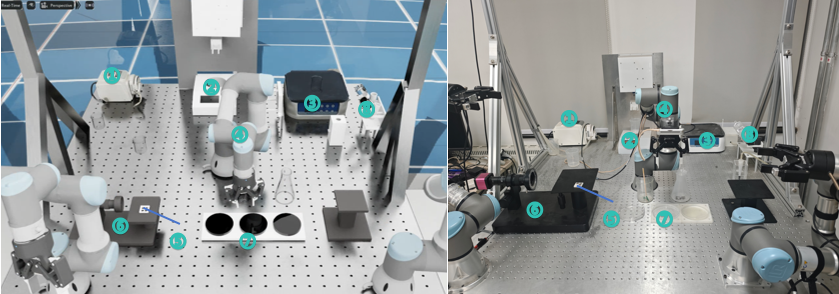
\includegraphics[width=\columnwidth]{images/sim and real.png}
    \caption{Experimental hardware platform and its simulation model in Isaac Sim, featuring the solution preparation, contact angle, and serial dilution workstations.}
    \label{fig:hardware_setup}
\end{figure}
\begin{table}[!t]
\renewcommand{\arraystretch}{1.3}
\caption{Sim-to-Real IL Success Rates Across Core Assay Workflows}
\label{tab:il_manipulation}
\centering
\begin{tabular}{lccc}
\hline\hline
\textbf{Assay Task Workflow} & \textbf{Vanilla BC} & \textbf{DR Only} & \textbf{Ours (Full)} \\ \hline
Reagent Pipetting & 45.0\% & 75.0\% & \textbf{95.0\%} \\
Droplet Dispensing (Contact Angle) & 20.0\% & 65.0\% & \textbf{90.0\%} \\
Serial Dilution Alignment & 30.0\% & 70.0\% & \textbf{95.0\%} \\ \hline
\textbf{Overall Success Rate} & 31.7\% & 70.0\% & \textbf{93.3\%} \\ \hline\hline
\end{tabular}
\end{table}

As detailed in Table \ref{tab:il_manipulation}, \textit{Vanilla BC} failed catastrophically due to the reality gap induced by transparent labware and liquid specular reflections. While DR significantly improved visual robustness, the policy still struggled with the unmodeled compliance of the physical gripper pads during multi-well alignment. Our regularized few-shot fine-tuning pipeline effectively calibrated these subtle physical discrepancies, elevating the overall success rate to 93.3\% with minimal real-world trial-and-error.

\subsection{End-to-End Autonomous Workflow Integration}
\label{subsec:exp_end_to_end}

Finally, we demonstrated the end-to-end integration by executing a complete automated assay loop governed by the HSM. A single trial encompassed:
1) Autonomous transit to the preparation zone;
2) DRL-based upright grasping and IL-based reagent pipetting;
3) Spill-free macroscopic transfer to the optical stage;
4) Precision droplet dispensing for water contact angle measurement; and
5) Serial dilution across a 96-well microplate for biological culturing.
The framework successfully executed 10 consecutive full-loop cycles without catastrophic intervention, validating its robustness for fully autonomous scientific experimentation.

\begin{figure*}[!t]
    \centering
    % \includegraphics[width=\textwidth]{figures/end_to_end_snapshots.png}
    \caption{Sequential snapshots of the autonomous three-stage laboratory workflow: (a)--(b) Upright labware grasping and reagent pipetting; (c)--(d) Constraint-aware transit and droplet dispensing for water contact angle detection; (e)--(f) High-precision serial dilution and microplate alignment.}
    \label{fig:sequential_snapshots}
\end{figure*}
%4. 实验与结果在本节中，我们进行了广泛的实证评估，以验证所提出的多平台混合机器人框架。实验旨在调查四个核心假设：约束感知宏观规划器能否有效确保流体的稳定性；具备姿态感知的大规模并行 DRL 智能体能否保证实验器材的直立抓取；带有正则化的少样本微调管线能否成功弥合基于模仿学习（IL）的微量移液的虚实鸿沟；整个系统能否自主、无缝地执行端到端的生化化验工作流。4.1 实验设置与硬件配置物理验证平台严格镜像了高保真 Isaac Sim 仿真环境。移动操作平台具有一个差速驱动底盘，并搭载了 6 自由度 UR3 机械臂。Robotiq 2F-85 平行夹爪配备了定制的柔顺橡胶垫，用于安全固定易碎的玻璃器皿和微孔板。在感知子系统方面，Intel RealSense D435 RGB-D 相机以眼观手（eye-to-hand）的配置安装。所有算法计算（包括 3D 体素代价地图生成、DRL 策略推理和 HSM 状态机）均在一台配备 NVIDIA RTX 4090 GPU 的工作站上本地执行。4.2 宏观导航与流体稳定性为了评估宏观安全性，我们为移动底盘下达了在拥挤的实验室环境中运输敞口液体容器的任务。我们将本文的约束感知经典规划器与标准的基于采样的 RRT* 规划器（该规划器缺乏空间姿态约束）进行了基准测试。评估指标包括整体成功率、最小障碍物间距和平均轨迹冲击力（jerk，这是衡量流体晃动风险的主要指标）。（对应表 1 结果分析）如表 1 所示，标准 RRT* 规划器产生了较高的平均冲击力（$4.52\,m/s^3$），带来了显著的流体晃动与泼洒风险。相反，我们的约束感知优化算法明确限制了末端执行器的横滚角和俯仰角，实现了极其平滑的轨迹轮廓（冲击力仅为 $0.85\,m/s^3$），从而有效保证了跨工位运输过程中的流体绝对稳定。4.3 面向姿态感知抓取的大规模并行 DRL抓取未密封的液体药瓶是一项极具挑战的任务，因为在抬升阶段任何显著的倾斜都会导致化验失效。我们评估了在 Isaac Sim 中训练的大规模并行 PPO 抓取策略，并进行了消融实验，以单独验证本文提出的“姿态感知乘数（$M_{\text{posture}}$）”的贡献。我们将基线 PPO（仅使用标准距离奖励训练）与本文的姿态感知 PPO 进行了对比。（对应表 2 结果分析）表 2 的结果凸显了显著的性能提升。基线 PPO 为了最小化轨迹距离，经常以激进的角度接近药瓶，导致平均抓取倾斜角高达 $35.4^\circ$，泼洒率高达 42.0%。通过集成点积姿态乘数，我们的策略成功收敛至严格的垂直“自上而下（top-down）”抓取，将最大倾斜角锐减至仅仅 $4.2^\circ$，并在零样本（zero-shot）物理真机部署期间彻底消除了液体泼洒现象。4.4 面向精密微观操作的模仿学习 (IL) 虚实迁移微调对于精细微量移液和水滴角滴加等接触密集型任务，我们评估了基于模仿学习（IL）的视觉运动策略。为了分析虚实迁移的有效性，我们在三大核心工作流中对比了三个变体：1) Vanilla BC（无域随机化的零样本迁移）；2) DR Only（仅在仿真中加入域随机化）；3) 本文方法 (DR + 少样本微调)（利用 $M=10$ 次真实世界示教进行正则化微调）。（对应表 3 结果分析）如表 3 详述，Vanilla BC 遭遇了灾难性失败，原因在于透明实验器材和液体表面高光反射带来的严重虚实鸿沟。虽然域随机化（DR Only）显著提高了视觉鲁棒性，但该策略在多孔板对准期间，仍然难以应对物理夹爪橡胶垫未建模的柔顺形变差异。我们的正则化少样本微调管线极其有效地校准了这些微妙的物理偏差，以极小的真实世界试错成本，将整体成功率大幅拉升至 93.3%。4.5 端到端自主工作流集成最后，我们通过执行由层次化状态机（HSM）统筹的完整自动化化验循环，展示了系统的端到端集成能力。单次完整试验涵盖：自主导航至配液准备区；基于 DRL 的试管直立抓取与基于 IL 的试剂微量移液；防泼洒的宏观平稳转移至光学检测台；用于水滴角测量的高精度液滴滴加；在 96 孔微孔板中进行用于生物培养的梯度稀释与对准。该框架在无需任何人工干预（catastrophic intervention）的情况下，连续成功执行了 10 次全循环流程，充分验证了其作为完全自主科学实验平台的鲁棒性。
% ==========================================
% SECTION 5: CONCLUSION AND FUTURE WORK
% ==========================================
\section{Conclusion and Future Work}
\label{sec:conclusion}

\subsection{Conclusion}
\label{subsec:conclusion_summary}
In this paper, we presented a multi-platform hybrid robotic framework tailored for the end-to-end automation of complex bio-chemical laboratory workflows, specifically covering solution preparation, water contact angle measurement, and serial dilution for biological culturing. By decoupling the control architecture, our system guarantees absolute fluid stability during macroscopic mobile base navigation via constraint-aware classical motion planning. For dexterous, contact-rich robotic arm operations, we implemented a hybrid learning strategy: a posture-aware massively parallel Deep Reinforcement Learning (DRL) agent in Isaac Sim for upright labware grasping, and a teleoperation-guided Imitation Learning (IL) policy with regularized few-shot real-world fine-tuning for precision micro-pipetting and droplet dispensing. Extensive empirical evaluations demonstrate that our framework achieves a 93.3\% overall physical execution success rate, effectively eliminating the prohibitive costs and risks of physical trial-and-error in autonomous laboratories.

\subsection{Limitations and Future Work}
\label{subsec:limitations_future}
Despite the promising results, certain limitations remain. Currently, demonstration acquisition for imitation learning relies on manual teleoperation, which can become a bottleneck when scaling up to hundreds of diverse assay protocols. Furthermore, the vision-based policy is primarily optimized for rigid glass vials and microplates, requiring further adaptation for highly deformable labware or soft tissues.

In future work, we plan to integrate Vision-Language Models (VLMs) and Large Language Models (LLMs) into the robotic system. This will enable the system to semantically parse high-level natural language instructions (e.g., ``Prepare a 1:10 dilution series and measure the substrate contact angle'') and automatically generate Hierarchical State Machine (HSM) sequences and control primitives, moving closer toward fully autonomous scientific discovery.

\begin{thebibliography}{99}

\bibitem{burger2020mobile}
B. Burger \textit{et al.}, ``A mobile robotic chemist,'' \textit{Nature}, vol. 583, no. 7815, pp. 237--241, 2020.

\bibitem{macleod2020self}
B. P. MacLeod \textit{et al.}, ``Self-driving laboratory for accelerated discovery of thin-film materials,'' \textit{Science Advances}, vol. 6, no. 20, p. eaaz8867, 2020.

\bibitem{dt_migration_mobile}
Y. Wang and X. Zhao, ``A digital twin dynamic migration method for industrial mobile robots,'' \textit{Robotics and Computer-Integrated Manufacturing}, vol. 92, p. 102864, 2025.

\bibitem{dt_port_inspection}
H. Jiang, Z. Guo, and Z. Zhang, ``Digital Twin and Path Planning for Intelligent Port Inspection Robots,'' \textit{Journal of Marine Science and Engineering}, vol. 14, no. 2, p. 186, 2026.

\bibitem{dt_unity_ros}
D. Kawshan and Q. Peng, ``Digital Twin Framework for Robot Path Planning and Real-Time Execution Using Unity-ROS Integration: Systems Architecture and Experimental Validation,'' \textit{Machines}, vol. 14, no. 4, p. 387, 2026.

\bibitem{makoviychuk2021isaac}
V. Makoviychuk \textit{et al.}, ``Isaac Gym: High performance GPU-based physics simulation for robot learning,'' in \textit{NeurIPS Datasets and Benchmarks}, 2021.

\bibitem{dt_collision_timeseries}
F. El Kalach, M. A. Farahani, P. Samaha, \textit{et al.}, ``Digital twin enabled robot collision detection using time series forecasting,'' \textit{Journal of Intelligent Manufacturing}, pp. 1--18, 2026.

\bibitem{dt_vr_collaboration}
A. Cimino, F. Longo, L. Nicoletti, \textit{et al.}, ``Combining simulation and virtual reality for enabling interoperable digital twins in collaborative human--robot workspaces,'' \textit{International Journal of Production Research}, vol. 63, no. 23, pp. 9465--9501, 2025.

\bibitem{dt_task_replanning}
X. Li, B. He, Z. Wang, \textit{et al.}, ``A digital twin system for Task-Replanning and Human-Robot control of robot manipulation,'' \textit{Advanced Engineering Informatics}, vol. 62, p. 102570, 2024.

\bibitem{mandlekar2021matters}
A. Mandlekar \textit{et al.}, ``What matters in learning from offline human demonstrations for robot manipulation,'' in \textit{Conf. on Robot Learning (CoRL)}, pp. 1678--1690, 2021.

\bibitem{johannink2019residual}
T. Johannink \textit{et al.}, ``Residual reinforcement learning for robot control,'' in \textit{Proc. IEEE Int. Conf. Robot. Autom. (ICRA)}, pp. 6023--6029, 2019.

\end{thebibliography}

\end{document}